\begin{figure*}[t!]
\centering
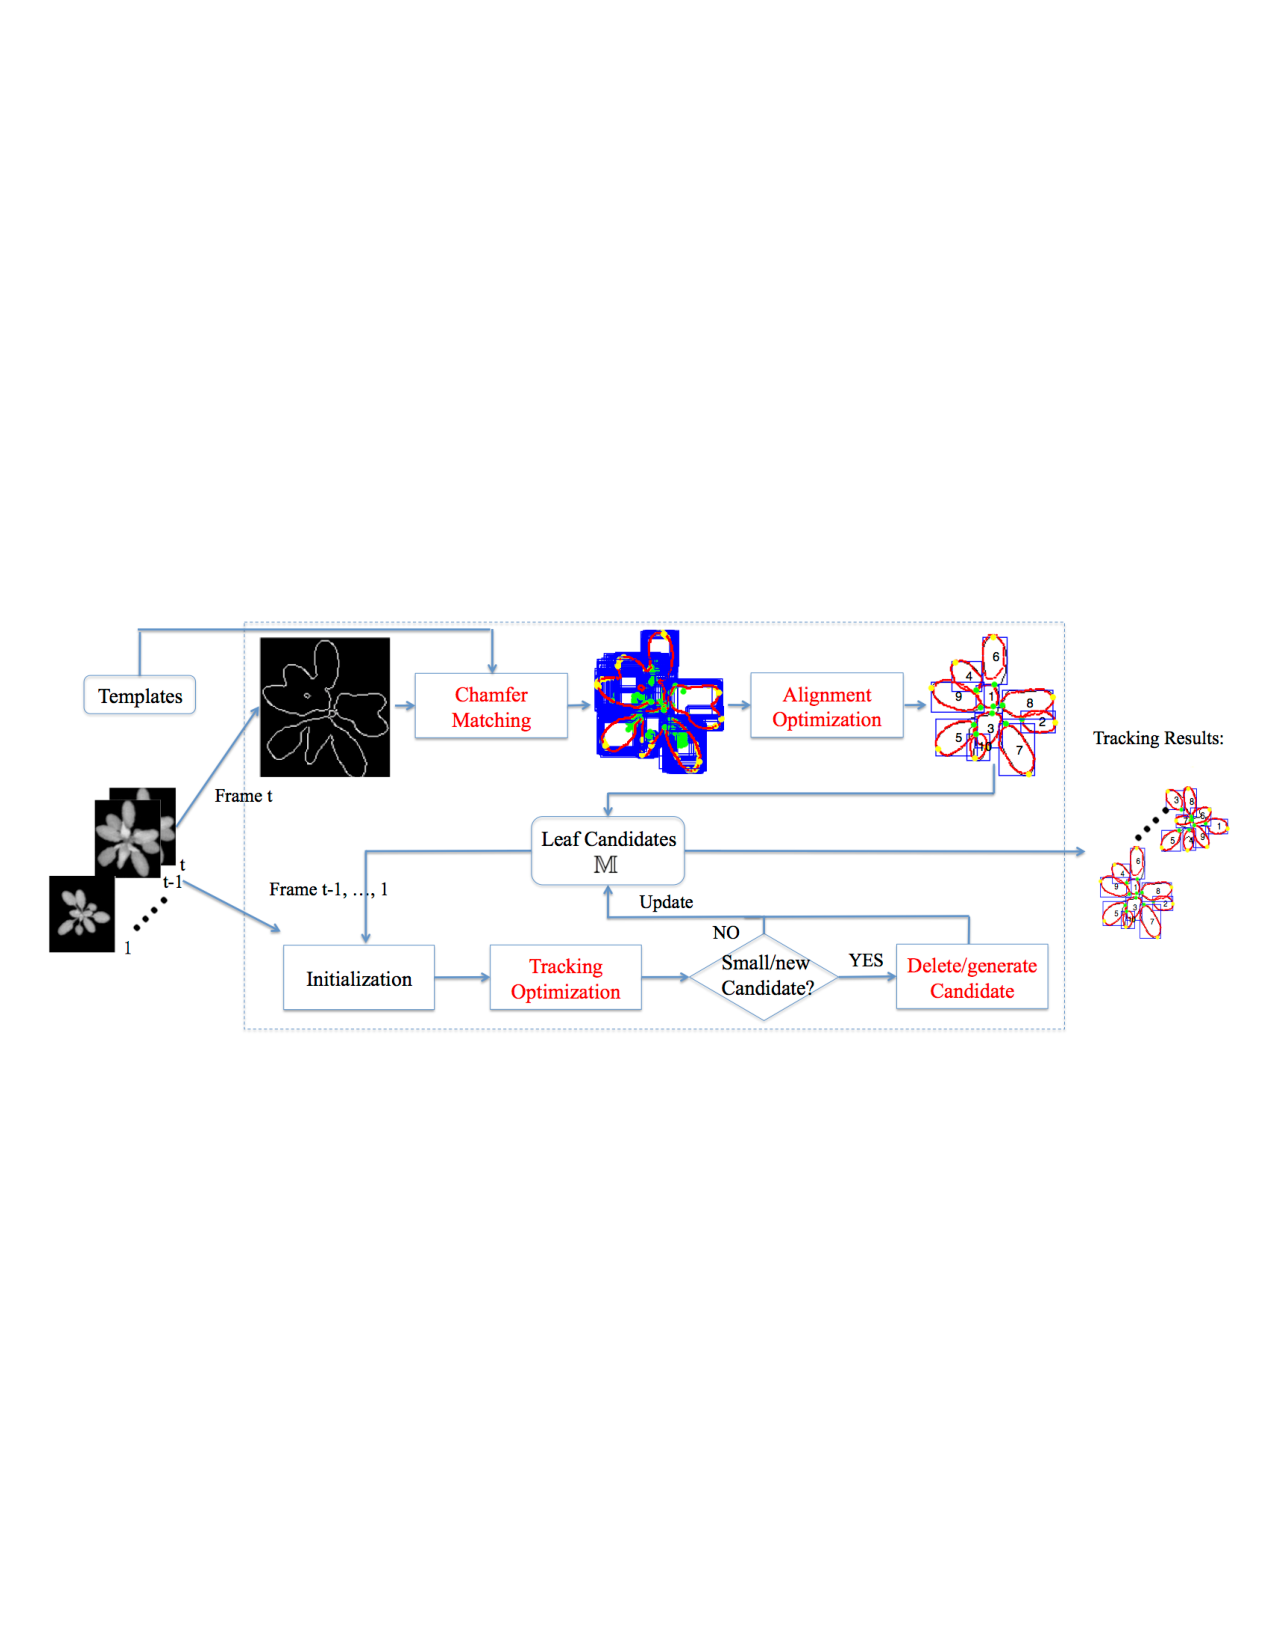
\includegraphics[width=.98\textwidth]{Figures/overview}\\
\caption{Overview of the baseline method.}
\label{fig:methodOverview}
\end{figure*}

\section{Baseline Method and Performance}
\label{sec:baseline}
\subsection{Our framework}
We apply our automatic multi-leaf segmentation and tracking framework~\cite{yin2014a,yin2014b} to the testing set of Arabidopsis fluorescence imagery to provide a baseline for future comparison.
Leaf segmentation aims at finding the correct number of leaves and the corresponding boundary of each leaf in each image.
Leaf alignment is to align the two tips of each leaf.
Leaf tracking is designed to track each leaf over time.




As shown in Fig~\ref{fig:methodOverview}, the input of this framework is a plant video and a set of predefined templates with various shapes, scales, and orientations.
To generate the template set, we first select $10$ templates with different aspect ratios from the labeled images in the training set together with the corresponding tip locations.
For each template, we scale it to $12$ different sizes in order to cover all size ranges in the database.
For each scale template, we rotated every $15^{\circ}$ to generate $24$ different directions.
Tip locations will be scaled and rotated accordingly.
Finally, we generate $2,880$ leaf templates.


%We also generate the two tips for each template for finding the corresponding tip points of each leaf via Chamfer Matching~\cite{barrow1977parametric}.
Our work is motivated by Chamfer Matching technique~\cite{barrow1977parametric}, which is used to align two edge maps.
We extend it to align multiple objects at the same time.
For each image, we use simple thresholding and edge detection to generate an edge map and mask.
First, we find the best location of each template in the edge map that has minimal chamfer matching distance, which will result in an over-complete set of leaf candidates.
Second, we apply multi-leaf alignment~\cite{yin2014a} approach to find an optimal set of leaf candidates on the last frame of the video, which will provide the information of the number of leaves, tip locations and boundaries of each leaf.
Third, we apply multi-leaf tracking~\cite{yin2014b} approach, which is based on leaf template transformation, to track leaves between continuous two frames.

In the tracking process, we develop a procedure to generate new leaves and delete small leaves.
For each frame of the video, we can generate a label image with each leaf being labeled with one color and the tip locations for each piece of leaf.
The label for each leaf in the video maintain the same during tracking process.


\subsection{Performance and analysis}
The results of our algorithm by varying $\tau$ from 0 to 1 is shown in Fig.~.
And the {\it{SBD}} score is $0.51$ by averaging over all plants.

\begin{figure*}
\centering
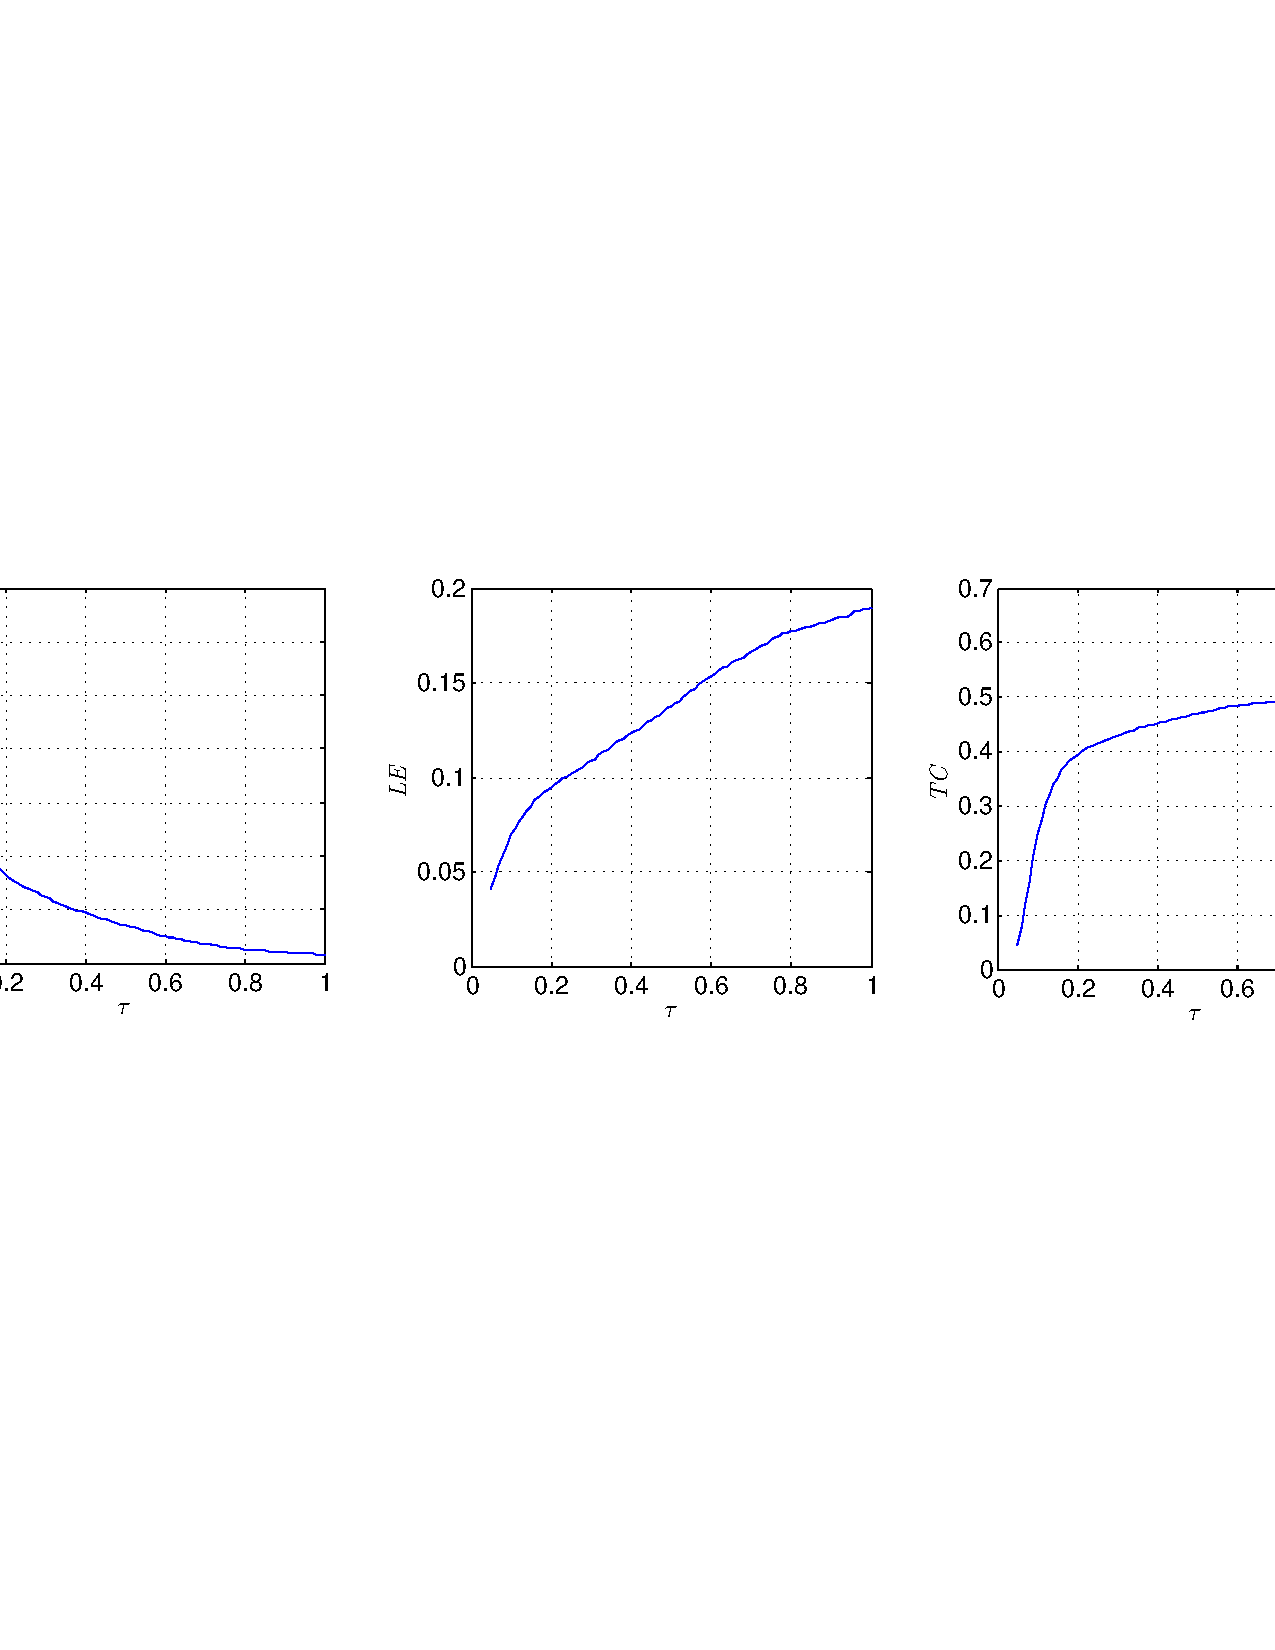
\includegraphics[width=.98\textwidth]{Figures/performance}\\
\caption{Performance of the baseline method.}
\label{fig:performance}
\end{figure*}



